\documentclass[../DoAn.tex]{subfiles}
\begin{document}

Chương 2 đã khảo sát, phân tích yêu cầu và chức năng cơ bản của hệ thống tích hợp dữ liệu so sánh giá. Chương này sẽ tập trung vào giới thiệu các công nghệ được sử dụng trong hệ thống. Bố cục chương sẽ chia thành các phần ứng với các pha khác nhau của luồng dữ liệu: (i) Hệ thống thu thập dữ liệu (Scrapy, Selenium), (ii) Hê thống lưu trữ và xử lý dữ liệu(Kafka, MongoDB, Python), (iii) Hệ thống tìm kiếm sản phẩm(Docker, React Js, Java Spring Boot).

\section{Thu thập dữ liệu}
\label{section:3.1}
\subsection{Scrapy}
\label{subsection:3.1.1}
Scrapy là một framework mã nguồn mở dùng để thu thập dữ liệu từ các trang web. Nó hỗ trợ việc thu thập dữ liệu một cách dễ dàng, tự động hóa quá trình thu thập và lưu trữ dữ liệu với các định dạng phổ biến như CSV, JSON hoặc XML. Scrapy còn cung cấp một hệ thống rất mạnh mẽ để quản lý request và response, cho phép bạn thực hiện việc lọc và xử lý dữ liệu dễ dàng. Nó cũng cung cấp một công cụ gọn nhẹ để tạo các spiders (chương trình) để thu thập dữ liệu từ các trang web.. Scrapy được sử dụng vơi nhiều mục đích khác nhau từ khai phá dữ liệu cho tới việc giám sát cũng như kiểm thử tự động trong nhiều hệ thống khác nhau.

% 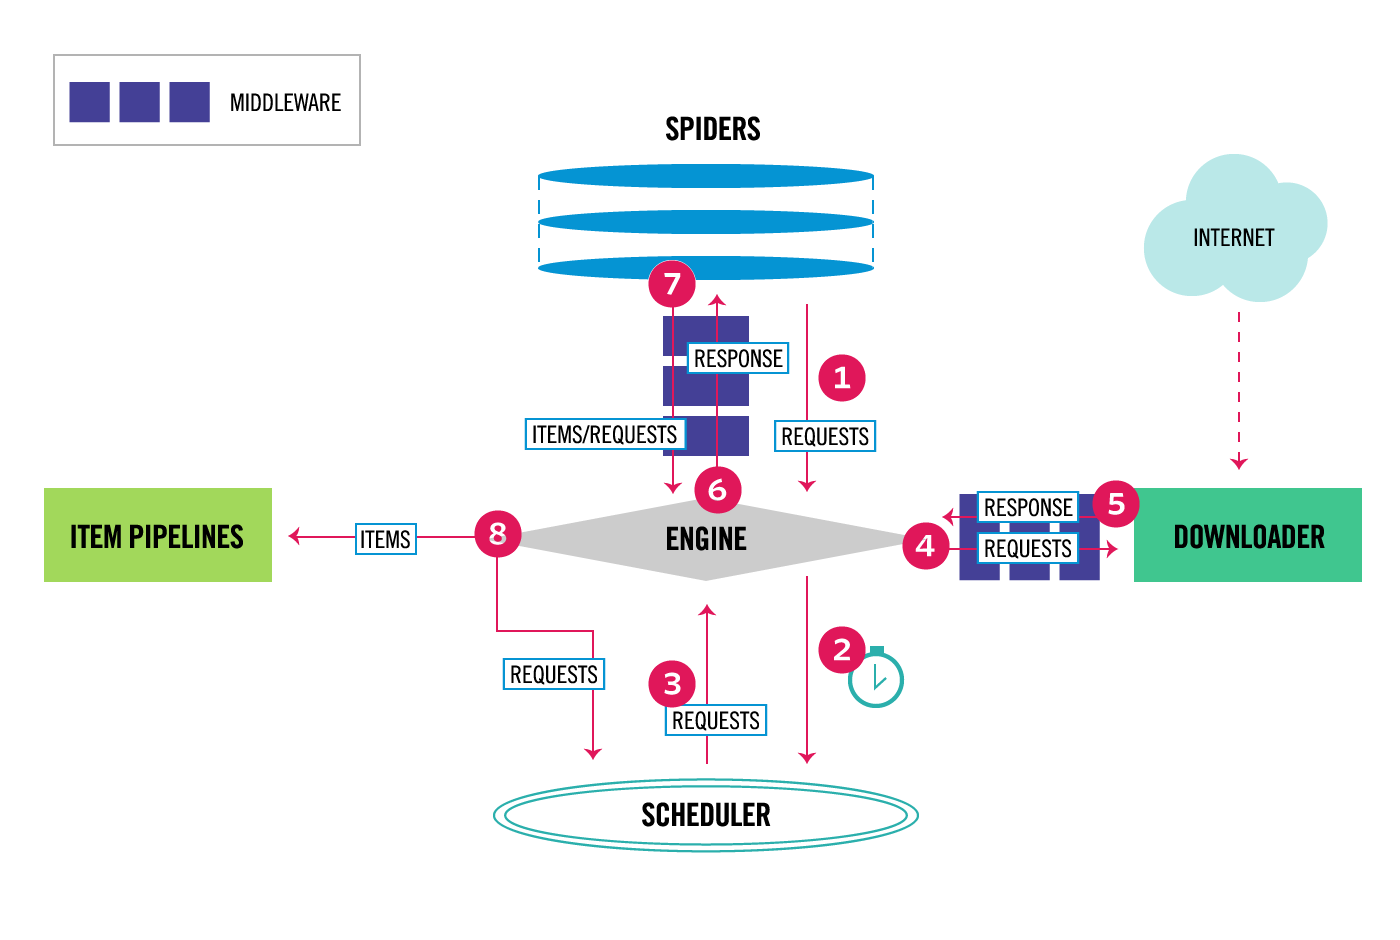
\includegraphics[scale=0.32]{Hinhve/scrapy_architecture.png}
\begin{figure}[H]
    \centering
    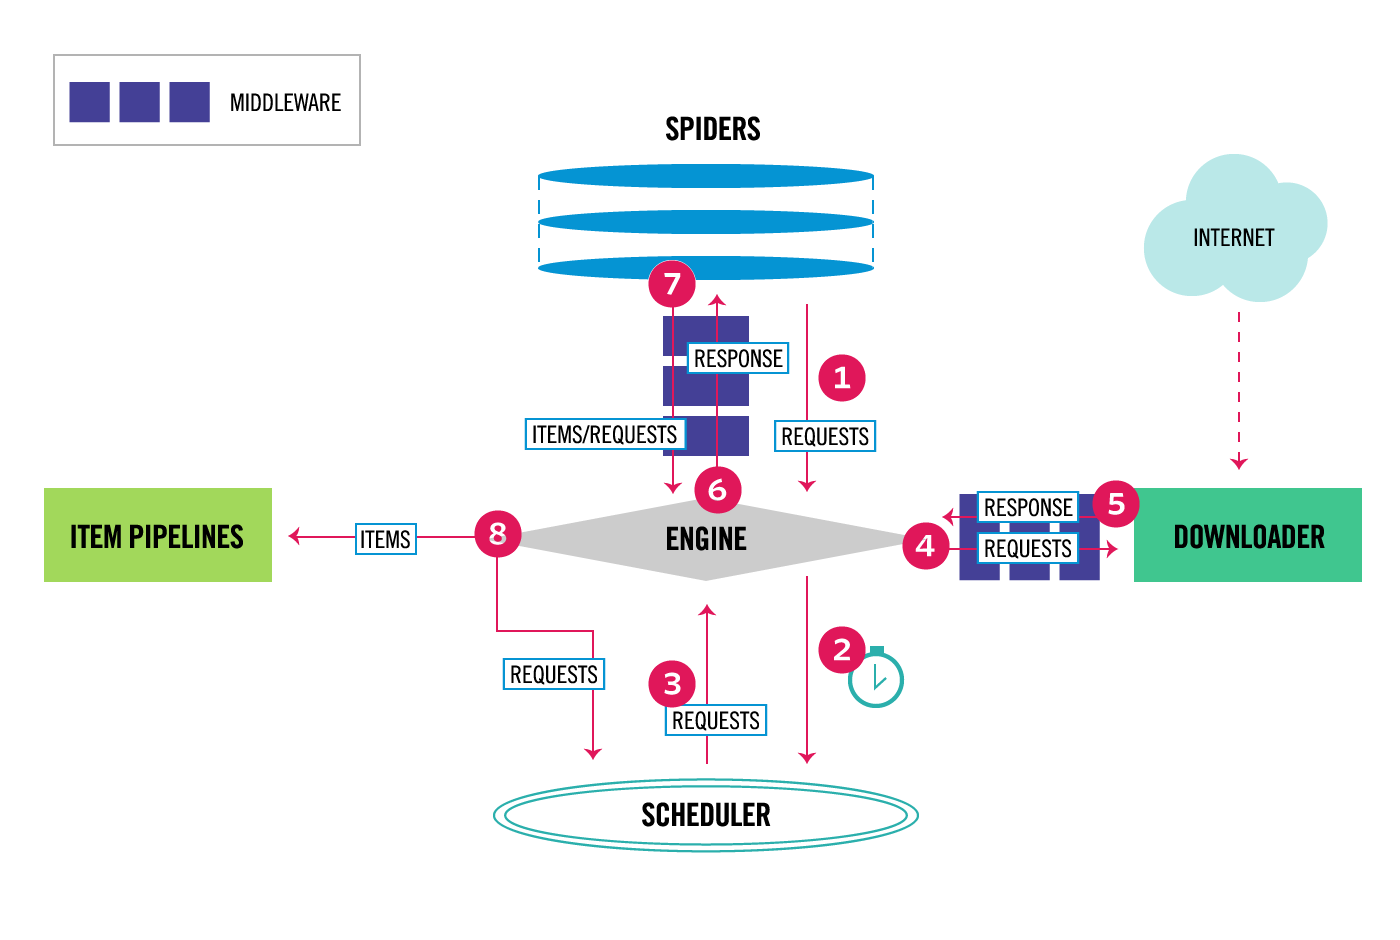
\includegraphics[scale=0.32]{Hinhve/scrapy_architecture.png}
    \caption{Kiến trúc của scrapy}
    \label{fig:my_label2}
\end{figure}

Kiến trúc của Scrapy framework gồm các thành phần chính sau:
\begin{itemize}
    \item Engine: Là nút chính của Scrapy, quản lý các hoạt động như thu thập dữ liệu, xử lý các request và response. Engine có trách nhiệm kiểm soát luồng dữ liệu giữa tất cả các thành phần của hệ thống và kích hoạt các sự kiện khi một số hành động xảy ra
    \item Schedule: Quản lý việc lấy các request từ độ ưu tiên và gửi cho Engine để xử lý
    \item Downloader: Thực hiện việc tải về các trang web từ Internet và trả về response cho Engine
    \item Spider: Là chương trình chính để thu thập dữ liệu từ các trang web. Spiders sử dụng các selector hoặc các công cụ xử lý HTML để trích xuất dữ liệu từ các trang web.
    \item Item Pipeline: Xử lý và lưu trữ các kết quả thu thập được từ các Spiders.
    \item Download Middleware: Là một tầng trung gian giữa Downloader và Engine, cho phép bạn thực hiện việc sửa đổi hoặc xử lý request và response trước khi chúng được gửi cho Spiders hoặc trước khi được lưu trữ
\end{itemize}

Scrapy hoạt động theo luồng dữ liệu khi bắt đầu crawl một website, Engine sẽ xác định tên miền và tìm vị trí của spider đó và yêu cầu spider đó tìm các urls đầu tiên để crawl. Engine nhận danh sách các urls đầu tiên từ spider, gửi cho Scheduler để sắp xếp Engine yêu cầu danh sách cách urls tiếp theo từ Scheduler Engine nhận danh sách các url tiếp theo từ Scheduler vào gửi đến Downloader (requests) Downloader nhận request và thực hiện việc tải trang, sau khi tải xong sẽ tạo một response và gửi lại EngineResponse từ Downloader sẽ được Engine đẩy qua Spiders để xử lýTại Spiders, khi nhận được response, chúng bóc tách thông tin từ response (title, content, author, date publish...) và những url có khả năngđể crawl và đẩy lại cho Engine (requests)Ở bước này, Engine nhận được kết quả từ Spiders sẽ thực hiện 2 côngviệc: đẩy những dữ liệu đã được bóc tách tới Item Pipeline để xử lý vàlưu vào Databases, đẩy những url mới (requests) mới về Scheduler và quay về bước 3.

\subsection{Selenium}
\label{subsection:3.1.2}
Selenium là một thư viện mã nguồn mở được sử dụng để tự động hóa việc điều khiển trình duyệt web và thu thập dữ liệu từ các trang web bằng cách tạo và chạy các đoạn mã tự động. Các đoạn mã này có thể truy cập các phần tử HTML trên trang web điền thông tin vào các mẫu và thực hiện các hành động như nhấp chuột, cuộn trang. Selenium thường được sử dụng để thu thập dữ liệu với mục đích phân tích hoặc khai thác dữ liệu từ các trang web động (trang web sử dụng javascript để hiển thị nội dung). Trong đồ án này em sử dụng thư viện Selenium để thu thập dữ liệu từ các trang web bán hàng trưc tuyến có chứa nội dung động.

% 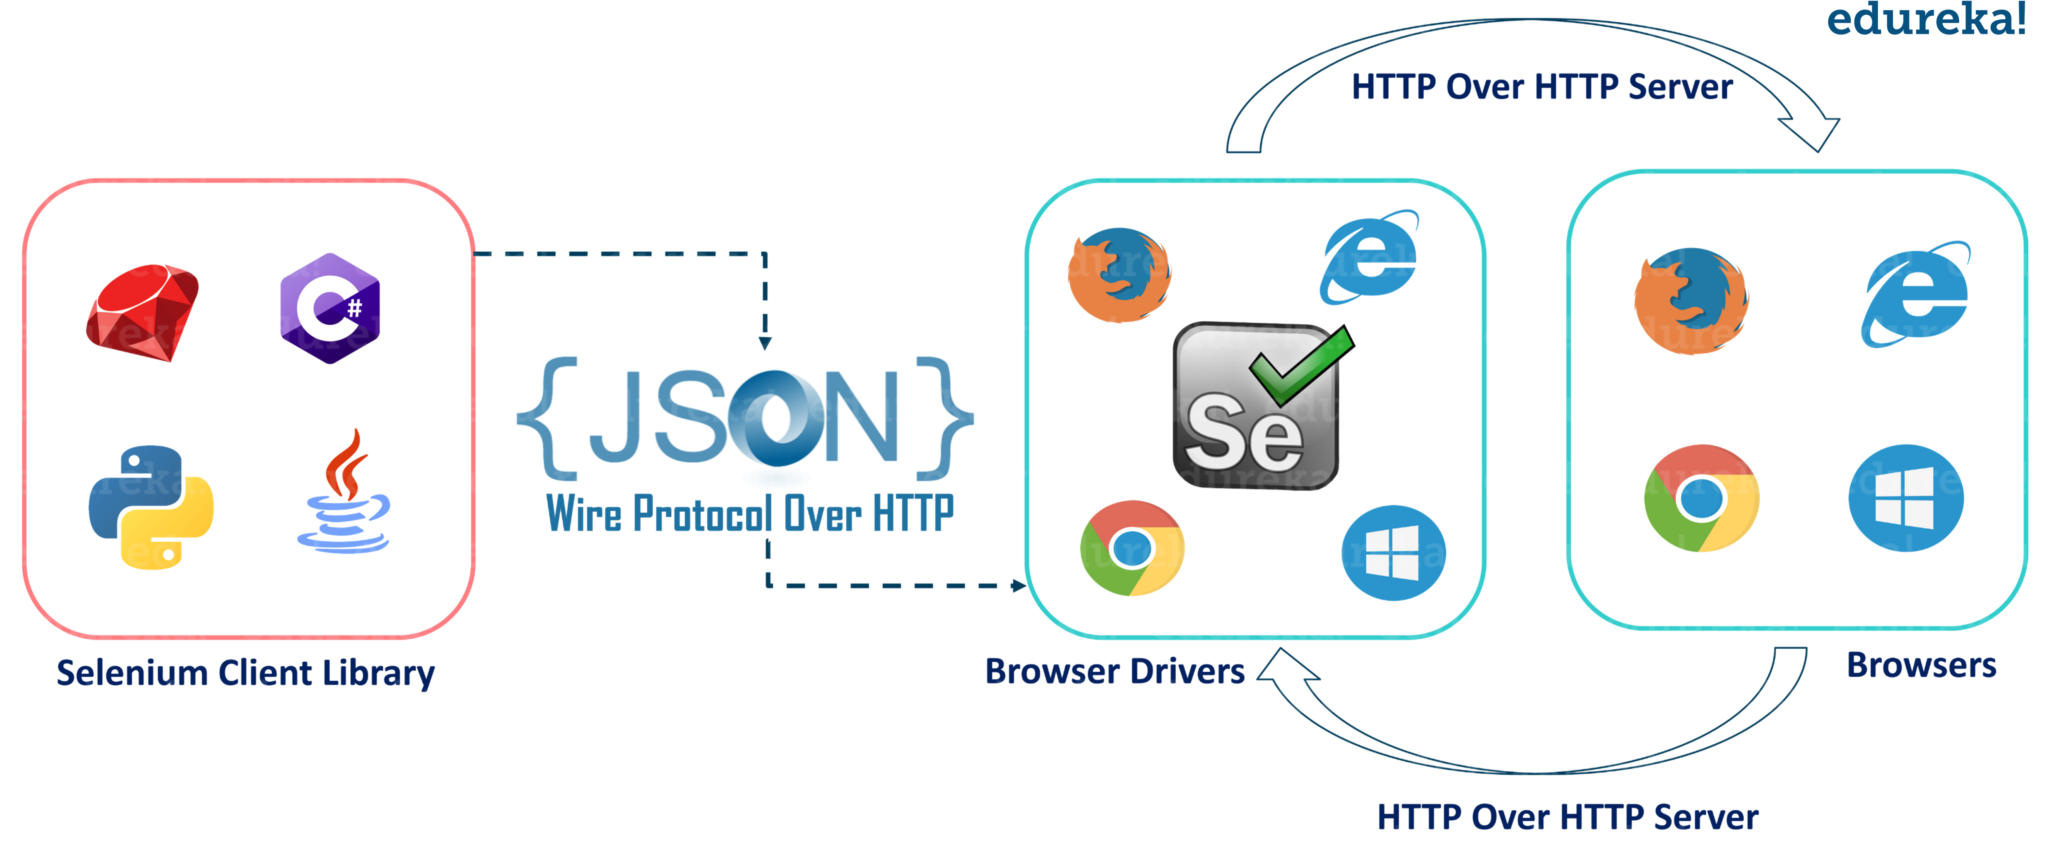
\includegraphics[scale=0.19]{Hinhve/selenium_architecture.png}
\begin{figure}[H]
    \centering
    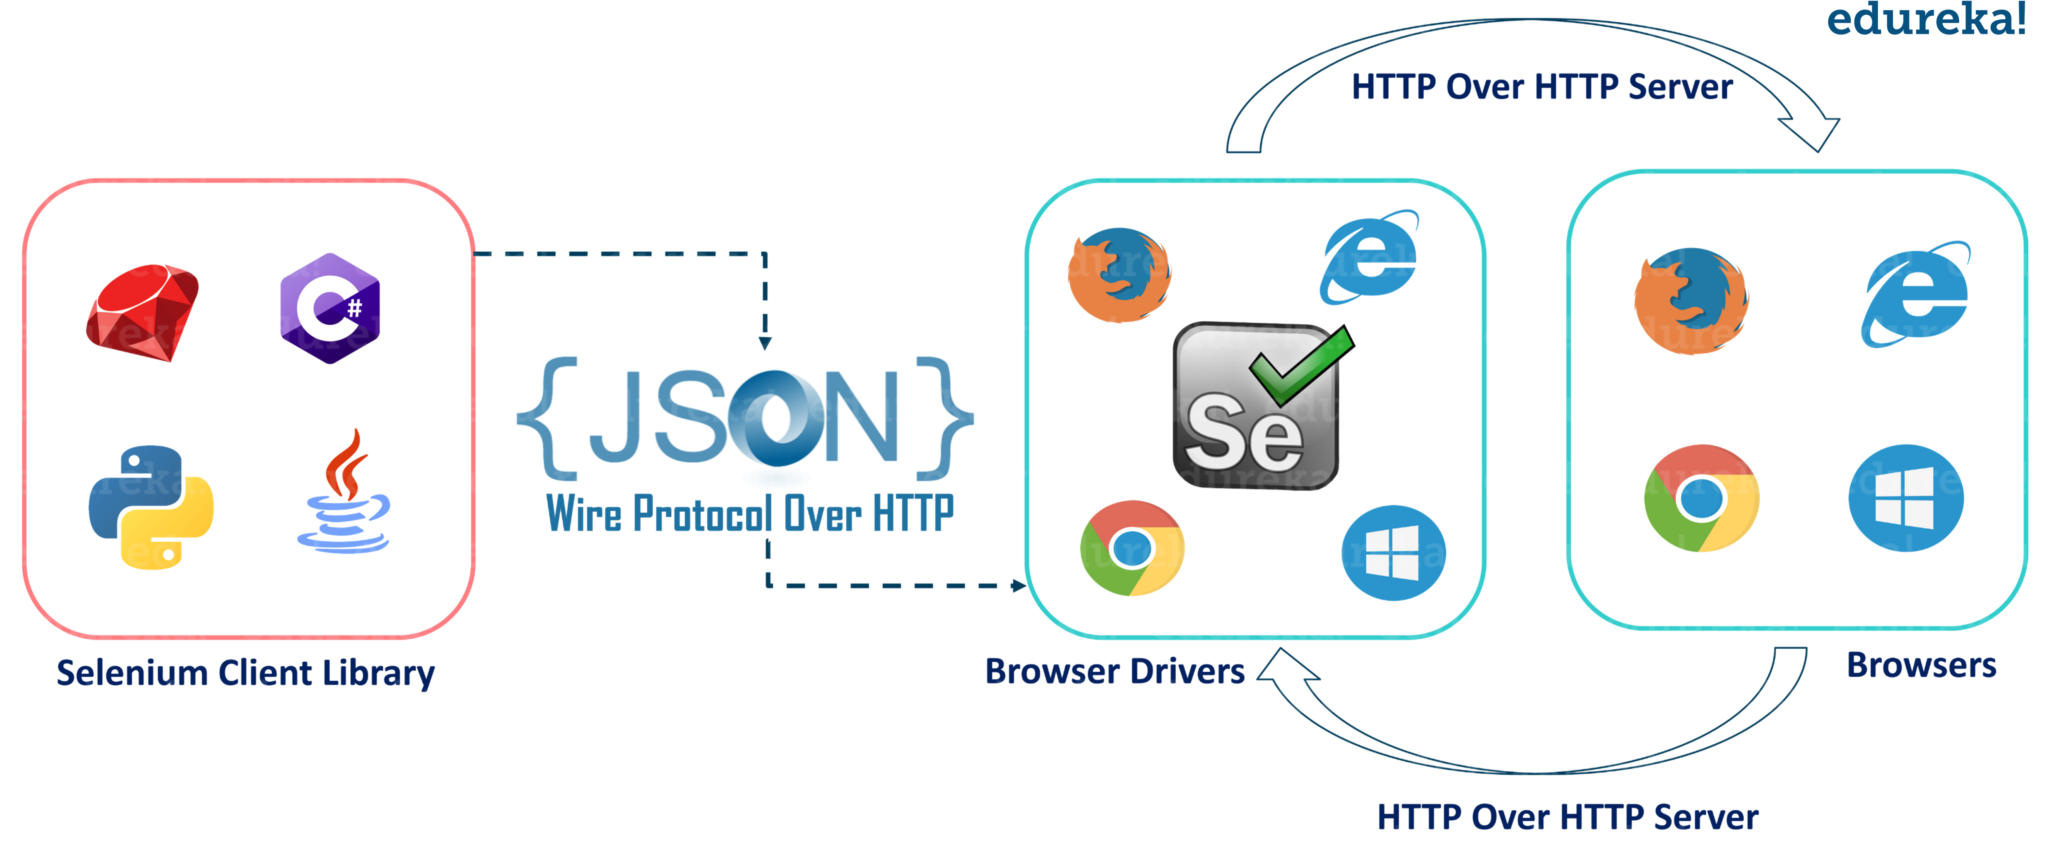
\includegraphics[scale=0.19]{Hinhve/selenium_architecture.png}
    \caption{Kiến trúc của selenium}
    \label{fig:my_label2}
\end{figure}

Kiến trúc của Selenium bao gồm các thành phần chính sau:
\begin{itemize}
    \item Selenium WebDriver: là thành phần chính của Selenium, đóng vai trò là giao diện giữa mã lập trình Python và trình duyệt web. Selenium WebDriver cho phép điều khiển các trình duyệt phổ biến như Chrome, Firefox, và Safari từ Python.
    \item Trình duyệt web: Selenium WebDriver sử dụng các trình duyệt web để tương tác với các trang web. Python có thể sử dụng với nhiều trình duyệt khác nhau như Chrome, Firefox, Safari, Opera và Edge.
    \item Selenium bindings cho Python: là các module Python cung cấp API để giao tiếp với Selenium WebDriver. Chúng cho phép lập trình viên tạo các script Python để điều khiển các trình duyệt web
    \item Test framework (khung kiểm thử): Nếu bạn sử dụng Selenium để kiểm thử ứng dụng web, bạn có thể sử dụng các framework kiểm thử như Pytest hoặc Unittest để tổ chức và thực hiện các bộ kiểm thử.
\end{itemize}
Với các thành phần này, lập trình viên có thể sử dụng Python API  để tạo các tương tác trên trình duyệt web, truy cập các phần tử HTML trên trang web để bóc tách XPath, Selectors thu thập dữ liệu từ các trang web.

\section{Hệ thống lưu trữ và xử lý dữ liệu}
\label{section:3.2}

\subsection{Apache Kafka}
\label{subsection:3.2.1}
Apache Kafka là một hệ thống mã nguồn mở và phân tán dùng để xử lý, lưu trữ và truyền tải luồng dữ liệu trực tiếp giữa các ứng dụng và dịch vụ. Kafka được thiết kế để có thể mở rộng và đồng thời giải quyết các vấn đề về tính độ tin cậy và hiệu suất trong việc xử lý lưu lượng dữ liệu lớn. Nó cho phép các ứng dụng ghi dữ liệu vào các topic và đọc dữ liệu từ các topic khác nhau, hỗ trợ thời gian thực và có tính đảm bảo, độ tin cậy cao. Kafka được sử dụng phổ biến trong các ứng dụng xử lý luồng dữ liệu, ghi nhật ký (logging), lưu trữ dữ liệu, phân tích thời gian thực, phân phối thông tin, hệ thống giao dịch tài chính và các ứng dụng Internet lớn. Với các tính năng của mình, Kafka đã trở thành một trong những công nghệ được ưa chuộng nhất để xử lý luồng dữ liệu trực tiếp.

Kafka được phát triển bởi Apache Software Foundation và được viết bằng Java, có thể hoạt động trên các hệ điều hành phổ biến. Nó cung cấp các tính năng như bảo mật, khả năng sao lưu và phục hồi dữ liệu, cơ chế phân phối và gom nhóm dữ liệu, và các giao diện lập trình ứng dụng (API) để phát triển các ứng dụng sử dụng Kafka. Trong hệ thống lưu trữ dữ liệu của đồ án em có sử dụng công nghệ này để lưu trữ dữ liệu sau khi được thu thập từ các trang web với mục đích lưu trữ với độ tin cậy cao, phân tích thời gian thực và cơ chế chịu lỗi tốt của nó.

\begin{figure}[H]
    \centering
    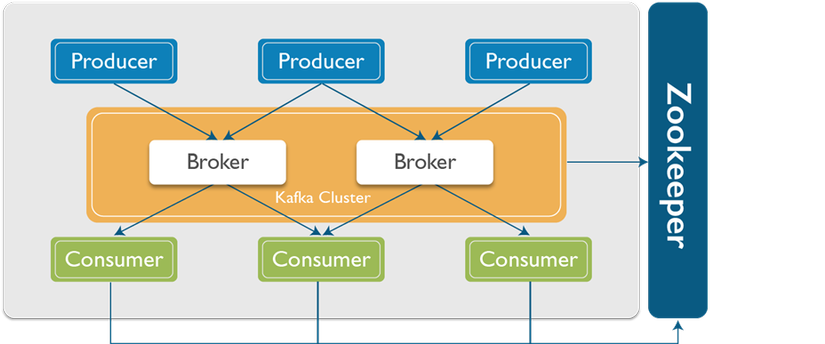
\includegraphics[scale=1.25]{Hinhve/kafka_architecture.png}
    \caption{Kiến trúc của kafka}
    \label{fig:my_label2}
\end{figure}

Kiến trúc của Apache Kafka bao gồm các thành phần chính sau:
\begin{itemize}
    \item Broker: Là một máy chủ Kafka chứa một hoặc nhiều topic và phân phối dữ liệu giữa các producer và consumer.
    \item Topic: Là một danh mục tương tự như một chủ đề, nơi dữ liệu được ghi và đọc. Mỗi topic được phân bổ trên nhiều partition để cho phép mở rộng dễ dàng.
    \item Partition: Là một phần của một topic và lưu trữ một phần của dữ liệu. Mỗi partition được lưu trữ trên nhiều broker để đảm bảo tính sẵn sàng và sao lưu.
    \item Producer: Là một ứng dụng ghi dữ liệu vào các topic và gửi chúng tới các broker để lưu trữ và xử lý.
    \item Consumer: Là một ứng dụng đọc dữ liệu từ các topic và xử lý chúng. Consumer có thể đọc dữ liệu từ nhiều partition để tăng hiệu suất.
    \item Group: Là một tập hợp các consumer có cùng một group ID để đọc dữ liệu từ một topic. Khi có nhiều consumer trong cùng một group, Kafka sẽ tự động phân phối các partition cho từng consumer để đảm bảo tính sẵn sàng và hiệu suất.
    \item ZooKeeper: Là một dịch vụ quản lý cấu hình và giám sát hệ thống Kafka. ZooKeeper giữ thông tin về trạng thái của các broker, partition, producer và consumer để đảm bảo tính đồng bộ và khả năng phục hồi.
\end{itemize}

Các thành phần này cùng hoạt động với nhau để tạo thành một hệ thống Kafka phân tán và đáng tin cậy cho việc xử lý, lưu trữ và truyền tải luồng dữ liệu.

\subsection{MongoDB}
\label{subsection:3.2.1}
MongoDB là một hệ quản trị cơ sở dữ liệu (DBMS) phi quan hệ mã nguồn mở, được phát triển bởi MongoDB Inc. MongoDB sử dụng mô hình lưu trữ tài liệu thay vì mô hình lưu trữ theo các bảng trong cơ sở dữ liệu quan hệ truyền thống. MongoDB là một cơ sở dữ liệu có khả năng mở rộng và phân tán, hỗ trợ các chức năng quản lý dữ liệu như tìm kiếm, truy vấn, phân trang và cập nhật. Nó cũng hỗ trợ nhiều ngôn ngữ lập trình khác nhau như Java, Python, Ruby, C# và PHP.
MongoDB có nhiều tính năng và lợi ích, bao gồm khả năng lưu trữ các tài liệu với các kiểu dữ liệu phong phú, cung cấp các tính năng bảo mật để bảo vệ dữ liệu, khả năng mở rộng dễ dàng với các cụm MongoDB, và hỗ trợ các tính năng thời gian thực như ghi log và thông báo thời gian thực.MongoDB được sử dụng rộng rãi trong các ứng dụng web, ứng dụng di động, Internet of Things (IoT), và các ứng dụng dữ liệu lớn. Trong đồ án này em có sử dụng MongoDB là cơ sở dữ liệu chính để lưu trữ dữ liệu sau khi xử lý và được truy vấn bởi hệ thống tìm kiếm yêu cầu phản hồi nhanh, truy vấn nhanh và lượng request lớn. 

% 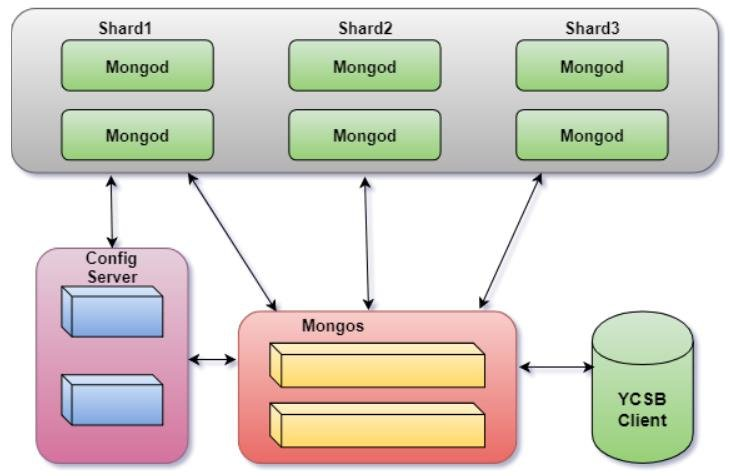
\includegraphics[]{Hinhve/mongodb_architecture.png}
\begin{figure}[H]
    \centering
    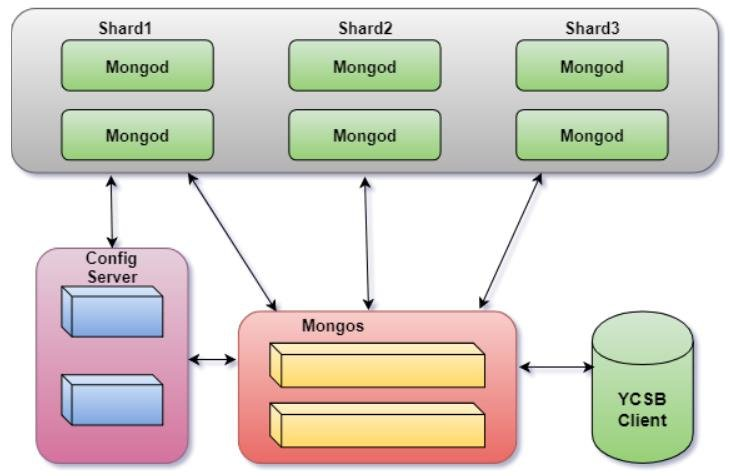
\includegraphics[]{Hinhve/mongodb_architecture.png}
    \caption{Kiến trúc của mongodb}
    \label{fig:my_label2}
\end{figure}

Các thành phần chính của hệ quản trị cơ sở dữ liệu phi quan hệ MongoDB:
\begin{itemize}
    \item Server: Thực thi các hoạt động truy vấn, quản lý các kết nối từ các ứng dụng và cung cấp khả năng mở rộng.
    \item Database: Là tập hợp các tài liệu được lưu trữ trên đĩa và được phân phối trên các máy chủ khác nhau.
    \item Collection: Là tập hợp các tài liệu có liên quan được lưu trữ trong cùng một vùng nhớ và có tên riêng biệt
    \item Document: Là đơn vị cơ bản của dữ liệu trong MongoDB, được biểu diễn dưới dạng JSON hoặc BSON, với các trường và giá trị tương ứng.
    \item Index: Là một cơ chế tìm kiếm nhanh cho các truy vấn, tăng tốc độ truy vấn.
    \item Replica set: Là một nhóm các bản sao dữ liệu, bảo đảm khả năng sẵn sàng và độ tin cậy cao.
    \item Sharding: Là một phương pháp phân tán dữ liệu trên nhiều máy chủ để đạt được khả năng mở rộng tốt hơn.
    \item Client: Là ứng dụng hoặc giao diện mà người dùng sử dụng để truy vấn và thao tác dữ liệu trong MongoDB.
\end{itemize}

\subsection{Độ đo khoảng cách Levenshtein}
\label{subsection:3.2.3}
Khoảng cách Levenshtein thể hiện khoảng cách khác biệt giữa hai chuỗi kí tự. Khoảng cách Levenshtein giữa hai chuỗi X và chuỗi Y là số bước nhỏ nhất để biến đổi chuổi X thành chuỗi Y hoặc ngược lại thông qua ba phép biến đổi cơ bản là thêm một kí tự, xóa một kí tự và thay thế kí tự này bằng kí tự khác. Để tính toán khoảng cách Levenshtein sử dụng thuật toán quy hoạch động tính toán trên mảng hai chiều (n+1)*(m+1) với n và m lần lượt là độ dài chuỗi A và B. Thuật toán chi tiết được minh họa sau đây

\begin{figure}[H]
    \centering
    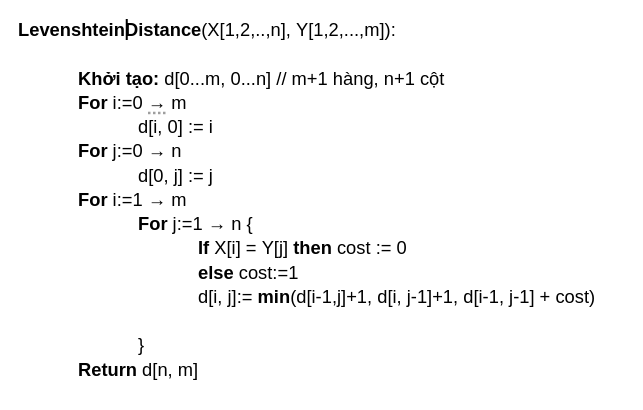
\includegraphics[scale=0.65]{Hinhve/levenshtein_algorithms.png}
    \caption{Thuật toán tính khoảng cách chỉnh sửa levenshtein}
    \label{fig:my_label2}
\end{figure}

Khoảng cách levenshtein là khoảng cách giữa hai chuỗi ký tự có giá trị d[n, m], với s là tổng độ dài của hai chuỗi kí tự độ đo tương tự được tính theo công thức sau:
\[sim(X, Y)= 1 - \frac{d[m, n]}{s}\]


\section{Hệ thống tìm kiếm }
\label{section:3.3}

\subsection{React Js}
\label{subsection:3.3.1}
React Js là một thư viện Javascript mã nguồn mở được phát triển bởi Facebook, ra mắt vào năm 2013 với mục đích để xây dựng giao diện người dùng. Nó được sử dụng rộng rãi để xây dựng các trang web ứng dụng một trang đơn SPA và các ứng dụng trên nền tảng di động. React Js dễ sử dụng cho phép người dùng có thể tạo các component UI có khả năng tái sử dụng. Một trong những điểm nổi bật của React là nó không chỉ hoạt động phía client mà còn render trên server và có thể kết nối với nhau. React so sánh sự khác nhau, thay đổi giữa các giá trị của lần hiển thị này với lần hiển thị trước cập nhật ít thay đổi nhất trên DOM.

% 
\includegraphics[scale=0.7]{Hinhve/reactjs.png}
\begin{figure}[H]
    \centering
    
\includegraphics[scale=0.7]{Hinhve/reactjs.png}
    \caption{React Js}
    \label{fig:my_label2}
\end{figure}

Hệ thống web tìm kiếm sử dụng React Js để xây dựng giao diện front end với mục đích làm cho ứng dụng trở nên nhanh hơn vì React JS sử dụng DOM ảo để cache cấu trúc dữ liệu trong bộ nhớ và chỉ những thay đổi cuối mới được cập nhật vào trong DOM trình duyệt. ReactJS cho phép tạo các component theo từng chức năng và có thể tái sử dụng theo nhu cầu làm cho việc bảo trì sau này trở nên dễ dàng hơn. Bên cạnh đó React JS là một thư viện mã nguồn mở nên dễ dàng tiếp cận và phát triển cho người mới bắt đầu tìm hiểu.
\subsection{Java SpringBoot}
\label{subsection:3.3.2}
Spring Boot là một framework Java được sử dụng để xây dựng ứng dụng web và các dịch vụ web RESTful. Nó là một phần của hệ sinh thái Spring Framework được phát triển bởi Pivotal. Spring Boot tập trung vào việc giảm thiểu sự cồng kềnh của việc cấu hình và triển khai ứng dụng Spring truyền thống bằng cách cung cấp một cách tiếp cận "tất cả trong một" cho việc xây dựng ứng dụng. Spring Boot cung cấp cho người phát triển các tính năng như cấu hình tự động, sử dụng những thư viện phổ biến, cung cấp môi trường phát triển chuyên nghiệp và quản lý phụ thuộc tự động. Điều này giúp giảm thiểu thời gian và công sức cần thiết cho việc cấu hình ứng dụng.

% 
\includegraphics[scale=0.6]{Hinhve/spring-boot-logo.png}
\begin{figure}[H]
    \centering
    
\includegraphics[scale=0.6]{Hinhve/spring-boot-logo.png}
    \caption{Spring boot logo}
    \label{fig:my_label2}
\end{figure}

Ngoài ra, Spring Boot cũng hỗ trợ mô hình MVC (Model-View-Controller) để xây dựng các ứng dụng web. Nó cung cấp cho người phát triển các tính năng như định tuyến (routing), xử lý yêu cầu HTTP, cung cấp API RESTful và quản lý tài nguyên tĩnh. Spring Boot được sử dụng rộng rãi trong các ứng dụng web và dịch vụ web RESTful. Nó là một framework mạnh mẽ và tiện lợi cho việc phát triển các ứng dụng Java trong môi trường sản xuất.
\subsection{Docker}
\label{subsection:3.3.3}

Docker là một nền tảng ảo hóa cấp phần mềm (containerization) cho phép người dùng đóng gói ứng dụng cùng với tất cả các phụ thuộc của nó (thư viện, tệp cấu hình, ...) vào một container độc lập với hệ thống. Container giúp đơn giản hóa việc triển khai và chạy ứng dụng trên nhiều môi trường khác nhau như máy tính cá nhân, server, cloud computing,... Với Docker, các container có thể được tạo ra và quản lý một cách đơn giản và dễ dàng bằng các tệp cấu hình (Dockerfile) để đóng gói các ứng dụng và phụ thuộc của nó thành các container. Các container có thể được chạy trên nhiều môi trường khác nhau, giúp giảm thiểu sự khác biệt về môi trường và giảm thiểu sự phụ thuộc vào các máy chủ cụ thể.

Docker cũng cung cấp một số công cụ quản lý và triển khai container, bao gồm Docker Compose và Kubernetes. Docker Compose cho phép người dùng định nghĩa và chạy nhiều container liên quan đến nhau như một ứng dụng. Kubernetes cung cấp một giải pháp để quản lý các container trong môi trường sản xuất với tính năng tự động mở rộng, quản lý tài nguyên và khả năng phục hồi sự cố. Docker đang được sử dụng rộng rãi trong ngành công nghiệp và cộng đồng phát triển phần mềm với nhiều lợi ích như tăng tính di động, khả năng phát triển và triển khai ứng dụng nhanh hơn, tăng tính nhất quán và dễ bảo trì. Trong phạm vi đồ án này em sử dụng Docker để triển khai cụm Kafka và hệ thống tìm kiếm giúp cho việc phát triển cũng như vận chuyển được dễ dàng hiệu quả hơn.

% 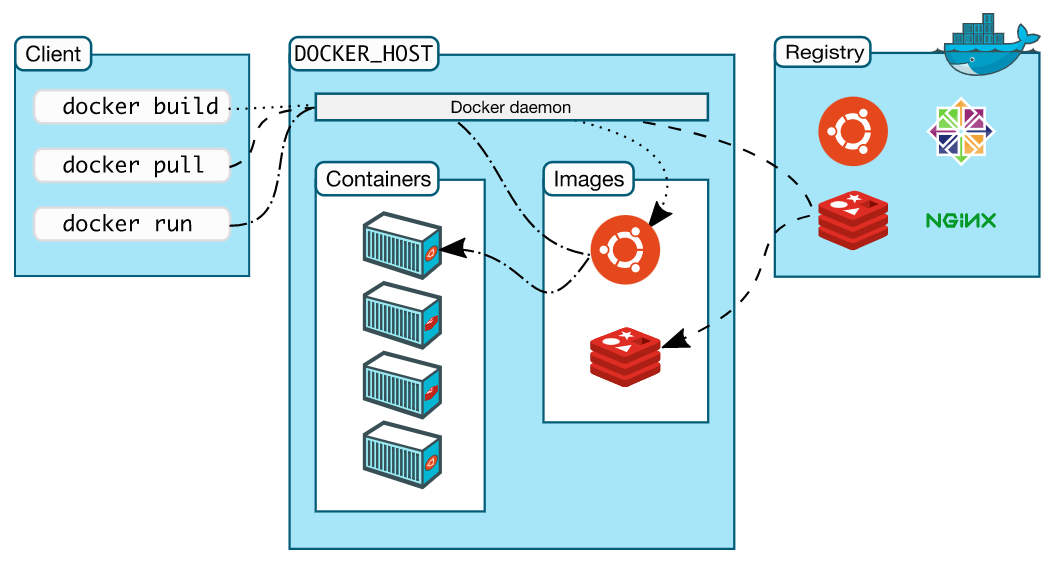
\includegraphics[scale=0.4]{Hinhve/docker_architecture.png}
\begin{figure}[H]
    \centering
    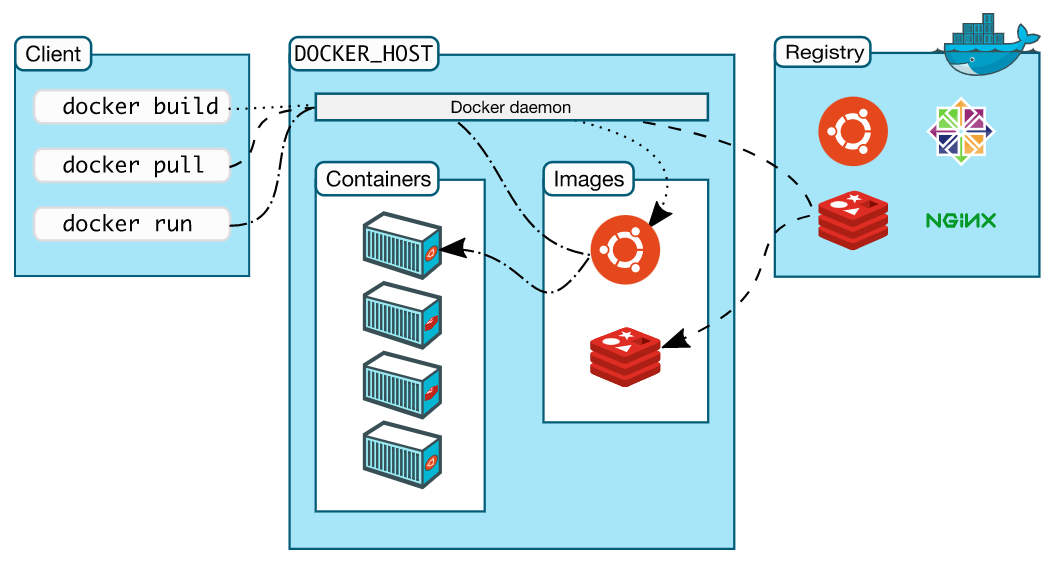
\includegraphics[scale=0.4]{Hinhve/docker_architecture.png}
    \caption{Kiến trúc của docker}
    \label{fig:my_label2}
\end{figure}

\begin{itemize}
    \item Docker Daemon: là một tiến trình chạy ngầm trên máy chủ và quản lý các container. Docker Daemon cung cấp API cho người dùng và Docker CLI để tương tác với các container.
    \item Docker CLI (Command Line Interface): là công cụ dòng lệnh cho phép người dùng tương tác với Docker Daemon và quản lý các container.
    \item Docker Images: là các bản đóng gói ứng dụng và tất cả các phụ thuộc của nó (thư viện, tệp cấu hình, ...) vào một container độc lập với hệ thống. Docker Images có thể được xây dựng từ các Dockerfile bằng cách sử dụng các lệnh để tạo và cấu hình các container.
    \item Docker Registry: là nơi lưu trữ các Docker Images. Docker Hub là một ví dụ của một Docker Registry công cộng, người dùng có thể tìm và tải về các Docker Images miễn phí từ đó
    \item Docker Container: là các container chứa các ứng dụng và phụ thuộc của nó. Docker Container được tạo ra bằng cách sử dụng Docker Images và được quản lý bởi Docker Daemon.
    \item Docker Network: cho phép các Docker Container trao đổi dữ liệu với nhau và với các ứng dụng khác trên cùng một mạng.
\end{itemize}

Docker cung cấp một kiến trúc mô-đun, cho phép các thành phần khác nhau của hệ thống được phân tách và quản lý độc lập với nhau. Docker cũng hỗ trợ việc tự động mở rộng và quản lý các container, đảm bảo tính sẵn sàng và tính nhất quán của hệ thống.

Chương này đã giới thiệu các công nghệ được sử dụng ứng với từng giai đoạn của hệ thống từ hệ thống thu thập dữ liệu, hệ thống lưu trữ và xử lý dữ liệu đến hệ thống tìm kiếm truy xuất dữ liệu. Các công nghệ trên đều đang được sử dụng phổ biến và đóng vai trò quan trọng trong nhiều hệ thống khác nhau. Việc xây dựng hệ thống dựa trên các công nghệ này được trình bày chi tiết ở chương tiếp theo đóng góp chính của đồ án.
\end{document}